\documentclass[11pt,a4paper]{article}
\usepackage[margin=1.9cm,top=1.7cm,bottom=1.8cm]{geometry}
\usepackage[T1]{fontenc}
\usepackage{lmodern}
\usepackage{microtype}
\usepackage{booktabs}
\usepackage{tabularx}
\usepackage{float}
\usepackage{array}
\usepackage{enumitem}
\usepackage{xcolor}
\usepackage{tikz}
\usetikzlibrary{positioning,fit,arrows.meta,backgrounds}
\usepackage[hidelinks]{hyperref}
\usepackage{titlesec}
\titlespacing*{\section}{0pt}{8pt}{3pt}
\titlespacing*{\subsection}{0pt}{6pt}{2pt}
\titleformat*{\section}{\large\bfseries}
\titleformat*{\subsection}{\normalsize\bfseries}
\setlist{nosep,leftmargin=1.2em}
\setlength{\parskip}{3pt}
\setlength{\parindent}{0pt}
\newcolumntype{Y}{>{\raggedright\arraybackslash}X}
\newcommand{\gh}[1]{\href{https://github.com/iDheer/tinydb/#1}}
\newcommand{\run}[1]{\href{https://github.com/iDheer/tinydb/actions/runs/#1}{#1}}
\renewcommand{\arraystretch}{1.12}

\begin{document}

{\Large\bfseries Architecting an Agentic SDLC Workflow: issue in, reviewed PR out}\\[2pt]
AutoSE Assignment 3 \quad·\quad Roll no.\ 2023111010 \quad·\quad
Fork \href{https://github.com/iDheer/tinydb}{iDheer/tinydb} (msiemens/tinydb @ \texttt{edff96a})
\quad·\quad Submission repo \href{https://github.com/iDheer/autose-a3}{iDheer/autose-a3}

\section{Architecture}

A GitHub Actions workflow (\texttt{.github/workflows/autose.yml}) turns an issue into a tested,
independently reviewed pull request in six fixed stages. A \textbf{deterministic Python state
machine} (\texttt{orchestrator.py}) owns the flow. Four LLM roles do the work. Agents propose
artifacts, code checks decide whether a stage passed, and a person decides whether to merge.
Agents never call GitHub and never hold a credential.

\begin{figure}[H]
\centering
\resizebox{\textwidth}{!}{%
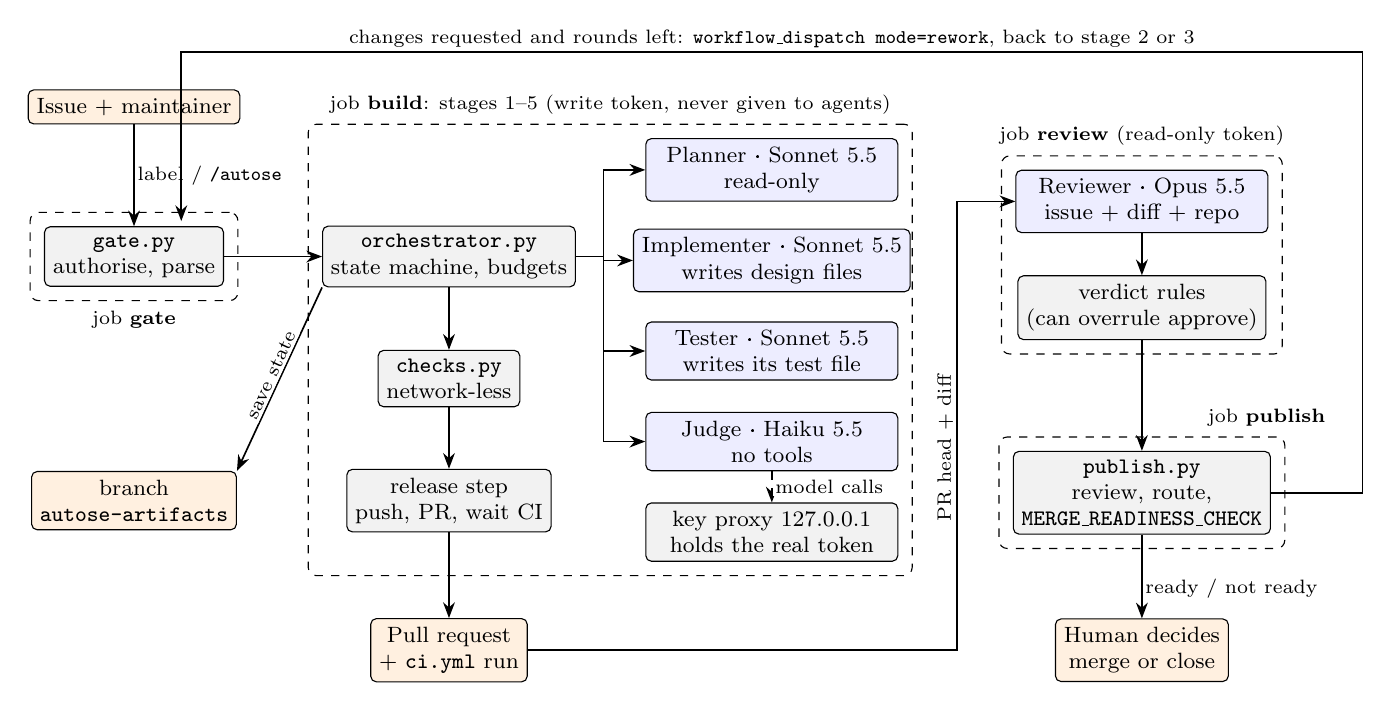
\begin{tikzpicture}[
  font=\footnotesize, x=1cm, y=1cm,
  box/.style={draw, rounded corners=2pt, align=center, inner sep=3pt, fill=white},
  agent/.style={box, fill=blue!7, minimum width=3.2cm},
  code/.style={box, fill=gray!10},
  ext/.style={box, fill=orange!12},
  job/.style={draw, dashed, rounded corners=3pt, inner sep=5pt},
  arr/.style={-{Stealth[length=2mm]}, semithick},
  lab/.style={font=\scriptsize, fill=white, inner sep=1pt}]
  \node[ext] (issue) at (0,0.3) {Issue + maintainer};
  \node[code] (gate) at (0,-1.6) {\texttt{gate.py}\\authorise, parse};
  \node[ext] (art) at (0,-4.7) {branch\\\texttt{autose-artifacts}};
  \node[code] (orch) at (4,-1.6) {\texttt{orchestrator.py}\\state machine, budgets};
  \node[code] (chk) at (4,-3.15) {\texttt{checks.py}\\network-less};
  \node[code] (rel) at (4,-4.7) {release step\\push, PR, wait CI};
  \node[agent] (plan) at (8.1,-0.5) {Planner · Sonnet 5.5\\read-only};
  \node[agent] (impl) at (8.1,-1.65) {Implementer · Sonnet 5.5\\writes design files};
  \node[agent] (test) at (8.1,-2.8) {Tester · Sonnet 5.5\\writes its test file};
  \node[agent] (judge) at (8.1,-3.95) {Judge · Haiku 5.5\\no tools};
  \node[code, minimum width=3.2cm] (proxy) at (8.1,-5.1) {key proxy 127.0.0.1\\holds the real token};
  \node[ext] (pr) at (4,-6.6) {Pull request\\+ \texttt{ci.yml} run};
  \node[agent] (rev) at (12.8,-0.9) {Reviewer · Opus 5.5\\issue + diff + repo};
  \node[code] (rules) at (12.8,-2.25) {verdict rules\\(can overrule approve)};
  \node[code] (pub) at (12.8,-4.6) {\texttt{publish.py}\\review, route,\\\texttt{MERGE\_READINESS\_CHECK}};
  \node[ext] (human) at (12.8,-6.6) {Human decides\\merge or close};
  \begin{scope}[on background layer]
    \node[job, fit=(gate), label={[font=\scriptsize]below:job \textbf{gate}}] {};
    \node[job, fit=(orch)(rel)(plan)(proxy), label={[font=\scriptsize]above:job \textbf{build}: stages 1--5 (write token, never given to agents)}] {};
    \node[job, fit=(rev)(rules), label={[font=\scriptsize]above:job \textbf{review} (read-only token)}] {};
    \node[job, fit=(pub), label={[font=\scriptsize]above right:job \textbf{publish}}] {};
  \end{scope}
  \draw[arr] (issue) -- node[lab, right]{label / \texttt{/autose}} (gate);
  \draw[arr] (gate) -- (orch);
  \foreach \a in {plan, impl, test, judge} \draw[arr] (orch.east) -- ++(0.35,0) |- (\a.west);
  \draw[arr] (orch) -- (chk);
  \draw[arr] (chk) -- (rel);
  \draw[arr, dashed] (judge) -- node[lab, right]{model calls} (proxy);
  \draw[arr] (orch.south west) -- node[lab, sloped, above]{save state} (art.north east);
  \draw[arr] (rel) -- (pr);
  \draw[arr] (pr.east) -- (10.45,-6.6) -- node[lab, sloped, above, pos=0.45]{PR head + diff} (10.45,-0.9) -- (rev.west);
  \draw[arr] (rev) -- (rules);
  \draw[arr] (rules) -- (pub);
  \draw[arr] (pub) -- node[lab, right, pos=0.65]{ready / not ready} (human);
  \draw[arr] (pub.east) -- (15.6,-4.6) -- (15.6,1.0) -- node[lab, above, pos=0.5]{changes requested and rounds left: \texttt{workflow\_dispatch mode=rework}, back to stage 2 or 3} (0.6,1.0) -- (0.6,-1.15);
\end{tikzpicture}}

\caption{Component view. Dashed boxes are Actions jobs, each with its own token permissions; blue
boxes are agents. Full view with every edge: \texttt{architecture/views/component-view.md}.}
\end{figure}

\vspace{-4pt}
\begin{table}[H]
\centering\scriptsize
\begin{tabularx}{\textwidth}{@{}l p{2.7cm} p{1.6cm} Y p{2.9cm}@{}}
\toprule
\# & Stage (agent) & Artifact & Check (code decides) & On failure \\
\midrule
1 & Requirements (Planner, A1 skill) & spec.md & Given/When/Then for every MUST/SHOULD criterion, no TBD or vague word, no open P1 question; Haiku judge rates each criterion testable & 1 retry; DRAFT $\to$ ask on issue, stop \\
2 & Design (Planner, A2 ARCHITECTURE.md) & design.md & named files exist; named functions/classes/methods exist (AST); every criterion mapped to code and a test idea & 1 retry \\
3 & Implementation (Implementer) & diff.patch & only design files changed; compileall, import, mypy & retry ($\le$3 per design) \\
4 & Testing (Tester) & test\_report.md & full suite passes; one test per criterion; $\ge$1 new test fails on base & $\to$ stage 3; then $\to$ stage 2 once \\
5 & Release (code) & pr.md + PR & PR open, \texttt{ci.yml} on the head commit succeeds & $\to$ stage 3 once with CI log \\
6 & Review (Reviewer, own job) & review.md & approve that survives the verdict rules, or 2 send-backs used & $\to$ stage 2 or 3, new run \\
\bottomrule
\end{tabularx}
\caption{Stage table (\texttt{architecture/views/stage-map.md}).}
\end{table}
\vspace{-6pt}

\textbf{Control flow and loops.} Stages 1--5 run in one \texttt{build} job. Transitions depend only
on check results and budget counters (\texttt{.autose/config.toml}). An agent can \emph{ask} for a
transition: the implementer can return \texttt{design\_gap} or \texttt{test\_dispute}. The
orchestrator grants the request only if the budget allows it. The review loop re-enters the workflow
by \texttt{workflow\_dispatch} with \texttt{mode=rework}. This is needed because a
\texttt{GITHUB\_TOKEN} push cannot trigger other workflows. Each issue has its own concurrency group.
State that must survive a restart (\texttt{state.json}, every artifact, every transcript) is
committed to an orphan branch \texttt{autose-artifacts}.

\textbf{Safety.} Only OWNER/MEMBER/COLLABORATOR comments or labels start a run. The issue text
reaches only the spec planner and the reviewer, inside an \texttt{<untrusted\_issue>} block with a
nonce. Agents talk to a local \emph{key-injecting proxy} with a dummy key, so neither they nor code
they run can read the real token. \texttt{GITHUB\_TOKEN} is removed from the environment before any
agent starts. Every tool call goes through a per-role PreToolUse policy hook: read and write paths
are checked, Bash commands are allowlisted, and shell metacharacters are rejected. The hook runs
every allowed command in a \emph{bubblewrap jail} with no network, its own PID namespace, and a
read-only filesystem except the work tree (ADR-011). Before pushing, the diff is secret-scanned.

\textbf{One real run} (sequence view: \texttt{architecture/views/sequence-view.md}). For issue
\gh{issues/1}{\#1}, run \run{43717026729} took 5\,min 18\,s. The judge rejected one
criterion whose Given relied on unstated data, so the spec was retried and passed. Design, code and
tests (4 tests, 2 of them failing on base) passed first time. CI passed, and PR \gh{pull/12}{\#12}
was opened. The isolated Opus reviewer ran the full suite and its own 5-test probe and approved.
\texttt{publish.py} then posted \texttt{MERGE\_READINESS\_CHECK} and handed the PR to a person.

\section{Decisions}

\begin{table}[H]
\centering\scriptsize
\begin{tabularx}{\textwidth}{@{}l l Y Y Y@{}}
\toprule
ADR & Area & Decision & Main alternative rejected & What the runs showed \\
\midrule
001 & D1 split & 4 roles split by permission (Planner, Implementer, Tester, Reviewer) + Haiku judge & one agent per stage; one agent for everything & Exp.\ B: separate tester gave no measurable gain on these issues \\
002 & D2 control & deterministic state machine; agents request, checks decide; jobs = trust boundaries & LLM orchestrator; one job per stage & 6 of 8 loop types fired; ``blocked'' bug fixed (\#11) \\
003 & D3 hand-off & schema-validated JSON rendered to md; raw issue only to spec + reviewer & free-text hand-off; full transcript to next agent & 0 of 73 sessions failed to return valid output \\
004 & D4 state & orphan branch \texttt{autose-artifacts} + \texttt{state.json} & Actions artifacts only; PR comments & every number in this report rebuilt from it \\
005 & D5 tools & SDK built-ins behind PreToolUse policy; GitHub only via \texttt{gh} in code & MCP GitHub server for agents; free Bash & 53 denials in 73 sessions (44 pipes/redirects, 9 e.g.\ \texttt{git stash}); all recovered \\
006 & D6 models & Sonnet 5.5 build, Opus 5.5 review, Haiku 5.5 judge; per-call turn/USD/time caps & one model everywhere & total \$6.31 for 73 sessions \\
007 & D7 checks & code checks; LLM only for testability & LLM judge for every stage & caught 2 vague ACs, 1 unmapped design, 2 CI failures \\
008 & D8 reviewer & own job, read-only token, issue + diff only, other model, verdict rules & reviewer sees spec/design/PR text & Exp.\ A: isolation routed better; equal catches \\
009 & D9 safety & key proxy, token scrub, untrusted fencing, 3 budget levels & key in agent env & \emph{superseded in part} by 011 \\
010 & D10 triggers & label or \texttt{/autose} by maintainer; queue per issue & any issue opener & gate ignored a malformed command (\run{43717817770}) \\
011 & D9 sandbox & own bubblewrap jail via hook (replaces SDK sandbox) & SDK weaker nested sandbox & SDK sandbox failed on runner (\run{43716337981}) \\
\bottomrule
\end{tabularx}
\caption{Decisions (Nygard-format ADRs in \texttt{architecture/decisions/}; superseded text is kept and marked).}
\end{table}
\vspace{-8pt}

\subsection*{Top decision 1: a deterministic state machine decides; agents only propose (ADR-002, ADR-007)}
\textbf{Why.} The six stages and their checks are fixed by the assignment, so routing does not need
judgement. An LLM orchestrator would add a failure mode (it can skip a check or loop) and buys
nothing. In code, every transition is a pure function of the check result and a counter. That makes
the loop bound provable: at most 3 implementation attempts per design, 1 design revision, 1 test
dispute, 1 CI retry and 2 review send-backs. It also lets each check be unit-tested without a model.
\textbf{Trade-off.} The state machine cannot handle situations it was not written for. If a run
leaves the expected path, it stops and posts the reason. It does not improvise.
\textbf{Evidence.} Six of the eight loop types fired in real runs:
\begin{itemize}
\item a spec retry after the judge's rejection (\#1, I3-selftest);
\item a needs-info stop and a restart after the maintainer's answer (\#5);
\item a design retry, a CI failure sent back to stage 3, and a test dispute sent to the tester (\#5);
\item a review send-back to stage 3, followed by an approval in round 2 (\#5).
\end{itemize}
Two loop types never fired: an implementation retry after a failed stage-3/4 check, and a design revision forced by test failures. Every implementation passed its checks first time. The one place where an agent's claim decided the outcome was a bug. The first run stopped because the
implementer \emph{said} it was blocked. I changed it so the check runs anyway (PR \gh{pull/11}{\#11}).

\subsection*{Top decision 2: the reviewer is isolated by job, token, context and model (ADR-008)}
\textbf{Why.} A reviewer that reads the implementer's summary, spec and design tends to check the PR
against those documents rather than against the issue, so it inherits their mistakes. The reviewer
therefore runs in its own job. Its token is \texttt{contents:read} only, and it sees only the issue,
the diff and the repository at the PR head. It uses another model (Opus 5.5), and its stance is to
find reasons not to merge. Code rules turn an approval into ``request changes'' in three cases: a
major or blocker finding exists, the full suite was not run, or a requirement has no evidence. The
review is posted as a COMMENT by a separate job, so it can never satisfy branch protection.
\textbf{Trade-off.} The reviewer pays to rediscover what the spec already says: an extra \$0.21--0.36
per review and 9--17 turns.
\textbf{Evidence.} Experiment A, §3. In the real runs, the reviewer found a regression on \#5 that
no hidden test covered: a user-supplied \texttt{cls=} encoder was silently overridden. Round 2
fixed it with tests.

\subsection*{Top decision 3: nothing worth stealing is in an agent's reach (ADR-009, ADR-011)}
\textbf{Why.} The input is untrusted issue text, and the agents run code. So the design assumes an
agent can be steered and limits what that achieves.
\begin{itemize}
\item The credential stays in a local proxy.
\item \texttt{GITHUB\_TOKEN} is popped before agents start.
\item Commands run with no network, in a jail where the orchestrator's processes and \texttt{/proc}
are invisible.
\item The reviewer cannot write anywhere that matters.
\end{itemize}
\textbf{Trade-off.} The proxy and the jail are my code on the critical path. \textbf{Evidence and
change.} ADR-009 relied on the SDK's Bash sandbox. On the GitHub runner it failed on every command
(\texttt{apply-seccomp: write /proc/self/setgroups: Permission denied}), which stopped the first real
run. Plain bubblewrap works there. So the policy hook now rewrites each allowed command to run under
\texttt{bwrap}. ADR-011 records this and marks ADR-009 as superseded in part; the original text is
kept. All later runs used the jail, and the build log shows the probe passing (``agent Bash jail:
bubblewrap'').

\section{Two tested decisions}
Each experiment changes one thing through a \texttt{workflow\_dispatch} input; everything else is
identical (\texttt{experiment/variants.md}). Results: \texttt{results/experiment\_A.csv},
\texttt{experiment\_B\_strength.json}, \texttt{runs.md}.

\noindent
\begin{minipage}[t]{0.488\textwidth}
\textbf{A. ADR-008: isolated vs.\ informed reviewer}\\[2pt]
\small
\textbf{Question.} Does hiding the spec, design and PR description make the reviewer catch more,
at the cost of more false alarms?\\
\textbf{Variant} \texttt{informed}: the reviewer also gets the PR description, spec.md and design.md.\\
\textbf{Subjects.} 5 seeded PRs (\gh{pull/6}{\#6}--\gh{pull/10}{\#10}). Two are correct (S1, S5).
Three have a known defect: S2, a generator consumed inside the lambda; S3, cache poisoning; S4, the
wrong approach. Each PR's own tests pass, and the descriptions are over-confident. 1 trial each.\\[3pt]
\scriptsize
\begin{tabular}{@{}lcc@{}}
\toprule
 & isolated & informed \\
\midrule
verdict = label & 4/5 & 4/5 \\
seeded defect named (S2--S4) & 3/3 & 3/3 \\
route correct (S2--S4) & \textbf{3/3} & 2/3 \\
S4 route (truth: design) & design & implement \\
false alarm on S1 & 0 & 0 \\
``false alarm'' on S5 & 1 & 1 \\
mean cost / turns & \$0.14 / 8.8 & \$0.17 / 8.4 \\
\bottomrule
\end{tabular}\\[3pt]
\small
\textbf{Reading.} Both variants caught every planted defect. On S3 both also found an unlabelled
second bug (on a cache hit, \texttt{limit} is ignored). Both flagged S5. The S5 finding is real:
with a negative limit, cached and uncached searches give different results. My label missed it.
The only difference between the variants was \emph{routing}. Shown the design, the informed
reviewer called the wrong-approach PR a code bug and would have sent it to stage 3 instead of
stage 2. It also judged details against the design (``design said keyword-only'') rather than the
issue. It cost 24\% more.\\
\textbf{Decision.} Keep the isolation, because it is cheaper and routes better. The evidence is
weak: one discordant PR out of five.
\end{minipage}\hfill
\begin{minipage}[t]{0.488\textwidth}
\textbf{B. ADR-001: separate tester vs.\ implementer's own tests}\\[2pt]
\small
\textbf{Question.} Do tests from an agent that never saw the implementer's reasoning catch more,
and is the extra session worth it?\\
\textbf{Variant} \texttt{selftest}: the implementer writes \texttt{tests/test\_autose\_issue\_N.py} in
the same session. The stage-4 check is unchanged, and the run stops after stage 4.\\
\textbf{Subjects.} I1--I4, 1 trial each. \textbf{Test strength}: run each test file against the
\emph{defective seeded implementation} of the same issue (S2/S3/S4).\\[3pt]
\scriptsize
\begin{tabular}{@{}lcc@{}}
\toprule
 & separate tester & selftest \\
\midrule
hidden tests passed & 13/13 & 13/13 \\
stage 3--4 iterations & 1 each & 1 each \\
own tests (I1/I2/I3/I4) & 4/6/11/3 & 5/6/12/7 \\
new tests failing on base & 2/3/8/3 & 3/3/9/7 \\
catch S2 / S3 / S4 & 3 / 2 / 3 fail & 3 / 2 / 7 fail \\
defect caught & 3/3 & 3/3 \\
cost to end of stage 4\textsuperscript{*} & --- & \$0.17--0.34 \\
\bottomrule
\end{tabular}\\
{\tiny * baseline costs include stage 5, so the build costs (\$0.21--0.33) are not directly comparable.}\\[2pt]
\small
\textbf{Reading.} This is a null result. Both variants fixed every issue on the first attempt, and
both test sets caught every seeded defect. The implementer even wrote more tests (I4: 7 vs.\ 3). On
issues this small, the implementer's assumptions did not leak into its tests in a way I could
measure. The separation matters most when the implementation is wrong, and here it was never wrong.\\
\textbf{Decision.} Keep the separate tester for now, because it is the cheap insurance in the
failure case that these runs never produced. I record that the data does not support it yet. If
larger issues also show no difference, merging stages 3 and 4 would save one session per round.
\end{minipage}

\section{Results}
\textbf{Runs.} 12 build runs, 6 issue reviews and 10 seeded-PR reviews, all on 2026-11-15. Every
run, PR and review is linked in \texttt{results/runs.md}; every row of \texttt{results.csv} is
rebuilt from \texttt{autose-artifacts} by \texttt{collect\_results.py}.

\noindent
\begin{minipage}[t]{0.47\textwidth}
\centering\scriptsize
\begin{tabular}{@{}l c l@{}}
\toprule
Stage & passed & failures \\
\midrule
1 Requirements & 10/13 & 2 vague ACs, 1 DRAFT \\
2 Design & 10/11 & 1 constraint not mapped \\
3 Implementation & 10/10 & --- \\
4 Testing & 12/12 & --- \\
5 Release (PR + CI) & 6/8 & 2$\times$ CI on Python 3.10 \\
6 Review & 5/6 & 1 real regression \\
\bottomrule
\end{tabular}\\[2pt]
{\scriptsize Pass rate per check evaluation, all 12 build runs (\texttt{stage\_checks.csv}).}
\end{minipage}\hfill
\begin{minipage}[t]{0.50\textwidth}
\centering\scriptsize
\begin{tabular}{@{}l c c l l@{}}
\toprule
Issue, PR & rounds & hidden & review & cost \\
\midrule
I1 bug, \gh{pull/12}{\#12} & 1 & 3/3 & approve & \$0.31+0.23 \\
I2 bug, \gh{pull/14}{\#14} & 1 & 3/3 & approve & \$0.22+0.21 \\
I3 feature, \gh{pull/15}{\#15} & 1 & 4/4 & approve & \$0.33+0.25 \\
I4 feature, \gh{pull/13}{\#13} & 1 & 3/3 & approve & \$0.21+0.25 \\
I5 vague, \gh{pull/17}{\#17} & 2 & 4/4 & changes$\to$approve & \$0.94+0.58 \\
\bottomrule
\end{tabular}\\[2pt]
{\scriptsize Final PR per issue (build + review cost). I5 includes the needs-info stop; I1 excludes
the failed first run (\$0.24).}
\end{minipage}

\textbf{Hidden tests.} I wrote 2--4 hidden tests per issue (17 in total), kept outside the fork. All
17 pass on the five final PRs, and the full suite stays green. All 13 for I1--I4 also pass on the
selftest diffs. The vague issue first stopped at stage 1 with three P1 questions. After my
maintainer answer it produced a PR that passes all 4 hidden tests. Those tests encode exactly the
answer: tz offset kept, date-like strings stay strings.

\textbf{Reviewer catches and misses.}
\begin{itemize}
\item \emph{Catches:} all 3 seeded defects in both variants, plus 1 unlabelled bug on S3, plus the
\texttt{cls=} regression on \#5, which the hidden tests did not cover.
\item \emph{Misses:} none against the hidden tests. None of the approved PRs fails a hidden test.
\item \emph{Disputed:} S5, where the reviewer was right and my label was wrong. I still count it as a
mismatch.
\item The reviewer \emph{did not} predict the Python 3.10 CI failure on \#5. It reviews after CI,
and its environment is Python 3.12.
\end{itemize}
Minor and nit findings were mostly real but low-value: missing docs for new API, untested
argument validation, an unused import.

\textbf{\texttt{MERGE\_READINESS\_CHECK}.} The assignment names this check but does not define it. I
implemented it as the last comment \texttt{publish.py} posts on every PR: a table of the stage checks
passed in the last build run, CI on the head commit, the independent verdict, the send-backs used,
the total model cost, and ``human decision required''. It ends with READY or NOT READY. All 5 issue
PRs ended READY FOR HUMAN REVIEW and carry \texttt{autose:ready-for-human}. None was merged.

\textbf{Cost and tokens.} The total is \textbf{\$6.31} at API list prices for 12 builds and 16
reviews, with no single run above \$0.55. Tokens: 574 uncached input, 257,940 output, 4,111,975
cache-read and 783,162 cache-write. Calls went through a Claude Pro subscription token with extra
usage off, which was the hard spending limit, so nothing was billed beyond the subscription.

\section{Hindsight}
\begin{itemize}
\item \textbf{Check the platform before trusting a security primitive.} I designed around the SDK
sandbox and unit-tested my policy locally. The first real run showed that the sandbox cannot start on
GitHub runners. I would now probe every isolation mechanism inside the workflow \emph{before} writing
the ADR.
\item \textbf{Give the agents the CI matrix.} Both CI failures came from one cause. The tester wrote
\texttt{import tomllib}, which needs Python 3.11, while CI also runs 3.10. The local stage-4 check runs
only 3.12, and round 2 reintroduced the same import. The stage-4 check should run the oldest
supported Python, and the matrix should be part of the tester's prompt.
\item \textbf{Artifacts must contain everything.} \texttt{git diff <base>} skips untracked files,
so the stage-4 \texttt{diff.patch} lost the new test file. I had to rebuild the experiment-B test
files from transcripts (PR \gh{pull/18}{\#18}). A check that each artifact is self-contained would
have caught this on day one.
\item \textbf{Use harder issues.} Every well-specified issue passed first time, so the loops were
exercised mostly by the vague issue. Experiment B could not separate its variants. The same budget
spent on fewer, harder issues would have taught more.
\item \textbf{Label seeded PRs adversarially.} The reviewer found a real defect in a PR I had labelled
correct. Ground truth should come from more than one reader.
\end{itemize}

\section{Limitations}
\begin{enumerate}
\item \textbf{Tiny samples.} 5 issues, 5 seeded PRs and 1 trial per cell. Experiment A's difference
is a single PR, and Experiment B is null. Neither supports a general claim.
\item \textbf{Author-made ground truth.} I wrote the issues, the hidden tests, the seeded defects and
the labels, and I judged ``defect named''. My blind spots are in the measuring stick: S5 shows the
labels can be wrong.
\item \textbf{Easy, well-structured repository.} tinydb is small and has strong tests, and the A2
architecture document names the invariants. Results on a larger codebase, with flaky tests or
multi-file features, could be very different.
\item \textbf{Correlated models.} The builders and the reviewer are from the same model family.
Shared blind spots would not show up as reviewer misses.
\item \textbf{Sandbox residue.} The jail hides the network, processes and \texttt{\$RUNNER\_TEMP}, but
the rest of the filesystem stays readable. The secret scan cannot catch an encoded exfiltration in a
committed file, so it relies on the jail having no network.
\item \textbf{Cost numbers are notional.} They are the SDK's list-price estimates. Subscription rate
limits, not money, bounded how much could run in parallel.
\end{enumerate}

\textbf{AI use.} Built with Claude Code (Opus 5.5): workflow and agent code, tests, issues, hidden tests,
seeded PRs, drafts of the ADRs, views and this report, and the demo video. The A1 skill and the A2
architecture document are my earlier work. I reviewed the decisions and results against the run
artifacts and redrew the diagrams.

\end{document}
